\documentclass{article}
%%!TEX encoding = UTF-8 Unicode
\usepackage[utf8]{inputenc}
%\usepackage{ngerman}
%\usepackage[ps2pdf,a4paper,colorlinks]{hyperref}
%\usepackage[a4paper,colorlinks]{hyperref}
\usepackage[a4paper]{hyperref}
\usepackage[a4paper,%
	inner=3.5cm,%
	outer=3.5cm,%
	top=4cm,%
	bottom=4cm,%
	marginparwidth=2.5cm,%
	marginparsep=0.3cm,%
	includehead]{geometry}
\usepackage{makeidx}
\usepackage[fleqn]{amsmath}
\usepackage{amsthm}
\usepackage{amstext}
\usepackage{amssymb}
\usepackage{mathtools}
\usepackage{xparse}
\usepackage{tikz}
\usetikzlibrary{automata,positioning}
% doesnt work?
%\usepackage{vaucanson-g}

\hypersetup{%
	pdftitle = {Language Operations and a Structure Theory of ω-Languages},%
	pdfsubject = {},%
	pdfauthor = {Albert Zeyer}%
}

% funktioniert nicht?
%\makeidx

%!TEX root =  index.tex

% some useful stuff:
% http://www.automata.rwth-aachen.de/material/skripte/latex/latex.pdf
% http://en.wikibooks.org/wiki/LaTeX/Mathematics
% http://en.wikibooks.org/wiki/LaTeX/Advanced_Mathematics
% http://en.wikibooks.org/wiki/LaTeX/Theorems

\newtheorem{thm}{Theorem}[section]
\newtheorem{lem}[thm]{Lemma}

\theoremstyle{definition}\newtheorem{mydef}{Definition}[section]
\theoremstyle{plain}\newtheorem{lemma}{Lemma}[section]
\theoremstyle{definition}\newtheorem{algo}{Algorithm}[section]

\newcommand{\K}{\mathcal{K}}
\newcommand{\Reg}{\text{Reg}}
\newcommand{\Lang}{\mathcal{L}}
\newcommand{\A}{\mathcal{A}}
\newcommand{\T}{\mathcal{T}}
\newcommand{\F}{\mathcal{F}}
\newcommand{\Q}{\mathbb{Q}}
\newcommand{\R}{\mathbb{R}}
\newcommand{\N}{\mathbb{N}}
\newcommand{\B}{\mathbb{B}}
\newcommand{\Power}{\mathcal{P}}

\newcommand{\mathtext}[1]{\textup{\textrm{#1}}}
\newcommand{\PT}{\mathtext{PT}}
\newcommand{\LT}{\mathtext{LT}}

% got some help here: http://tex.stackexchange.com/questions/13554/define-something-like-lim-but-for-another-name

\newcommand{\ext}{\operatorname{ext}}
\newcommand{\Inf}{\operatorname{Inf}}
\newcommand{\BC}{\operatorname{BC}}
\newcommand{\dext}{\operatorname{\overline{ext}}}
\newcommand{\dlim}{\operatorname{\overline{lim}}}
\newcommand{\Kleene}{\operatorname{\widehat{Kleene}}}
\newcommand{\limClosure}{\operatorname{\widehat{lim}}}
\newcommand{\Occ}{\operatorname{Occ}}
\newcommand{\existsinf}{\exists^\omega}
\newcommand{\overx}{\overset{\times}}
%\newcommand{\overx}{\stackrel{\times}}
\newcommand{\Ax}{\overx{\A}}
\newcommand{\Langreg}{\Lang^*(\text{reg})}
\newcommand{\LangOreg}{\Lang^\omega(\text{reg})}

\newcommand{\defword}[1]{{\bf #1}}

% inspired by http://ftp.fernuni-hagen.de/ftp-dir/pub/mirrors/www.ctan.org/macros/latex/contrib/braket/braket.sty
\def\mid@vertical{\mskip1mu\vrule\mskip1mu}
\def\midvert{\egroup\;\mid@vertical\;\bgroup}
\NewDocumentCommand\Set{mg}{%
    \IfNoValueTF{#2}{%
        \ensuremath{\left\{ #1 \right\}}%
    }{%
        \ensuremath{\left\{ {#1} \;\mid@vertical\; {#2} \right\}}%
    }%
}

%\newcommand{\SetS}[1]{\bigl\{ #1 \bigr\}}
%\newcommand{\SetC}[2]{\bigl\{ #1 \bigm| #2 \bigr\}}
%\DeclarePairedDelimiterX\SetC[2]{\lbrace}{\rbrace}{ #1 \,\delimsize|\, #2 }

%\newcommand{\abs}[1]{\mathopen| #1 \mathclose|}
%\newcommand{\Abs}[1]{\left| #1 \right|}
\newcommand{\abs}[1]{\left| #1 \right|}

% http://de.wikibooks.org/wiki/LaTeX-W%C3%B6rterbuch:_today
\def\monthgerman{\ifcase\month \or
  Januar\or Februar\or M\"arz\or April\or Mai\or Juni\or
  Juli\or August\or September\or Oktober\or November\or Dezember\fi}
\def\todaygerman{\number\day.~\monthgerman\space\number\year}


\begin{document}
\title{Language Operations and a Structure Theory of $\omega$-Languages}
\author{Albert Zeyer}
%\date{10. Februar 2011}
\date{\today}

\maketitle
\tableofcontents

%!TEX root =  index.tex

\section{Introduction}

The study of formal languages and finite-state automata theory is very old and fundamental in theoretical computer science. Regular expressions were introduced by Kleene in 1956 (\cite{Kleene56}). Research on the connection between formal languages, automata theory and mathematical logic began in the early 1960's by Büchi (\cite{Buchi60}). Good introductions into the theory are \cite{FinAutLogR109} and \cite{LangAutLogicR102}.

We call languages over finite words the $*$-languages. Likewise, $\omega$-languages are over infinite words. Words are just sequences of input symbols.

The class of regular $*$-languages is probably the most well studied language class. Its expressiveness is exactly equivalent to the class of finite-state automata as well as regular expressions. The connection between finite-state automata and regular languages was established by S. C. Kleene in \cite{Kleene56}. A more generic concept of finite-state automata, including the non-deterministic case, was introduced by M. O. Rabin and D. Scott in \cite{FinAutRabin59}. It was inspired as a strict subset of the Turing machine which has infinite many states given by its memory. Such finite-state automata get a sequence of input symbols and change their state on each input symbol. Depending on their state, we say that such automaton accepts a given word. Thus, an automaton is representing a language. And the class of languages given by such finite-state automata is equal to the class of regular languages.

For many applications, less powerful subsets of the regular $*$-languages are interesting, like starfree $*$-languages, locally testable $*$-languages, etc., as well as more powerful supersets, like context-free $*$-languages.

The research on $\omega$-languages and their connection to finite-state automata began a bit later by Büchi \cite{DecisionSOR111} and \cite{Muller63}. As for the $*$-languages, the most well studied $\omega$-language class are the regular $\omega$-languages. Good introductions into these theories are \cite{AutInfObjsR103}, \cite{InfCompR101}, \cite{OmLangR108} and \cite{InfWordsR110}. In contrast to the finite-word acceptance of automata, one can think of several different infinite-word acceptance conditions which lead to different automata, most importantly the Büchi and Muller automata. A central result by Robert McNaughton in \cite{McNaughton66} is the equivalence of non-deterministic Büchi automata and deterministic Muller automata.

Landweber established a strict hierarchy in \cite{Landweber69} on subsets of the regular $\omega$-languages, given by other/simpler infinite-word acceptance conditions in finite-state automata, namely the E-/A-acceptance condition and deterministic Büchi and co-Büchi automata.

For all types, we can also argue with equivalent language-theoretical operators which operate on a $*$-language and transform them into an $\omega$-language. We will study the equivalences in more detail. The most important operators are $\ext$, $\lim$, in some way equivalent to E-acceptance and deterministic Büchi acceptance, and boolean combinations of those. For some $*$-language $L$, $\ext L$ are all infinite words where some prefix is in $L$ and $\lim L$ are all finite words where infinitely many prefixes are in $L$.

Depending on the $* \rightarrow \omega$ language operator or the $\omega$-automaton acceptance condition, we get different $\omega$-language classes. This was studied earlier already in detail for the class of regular $*$-languages. E.g., we get the result that the class of boolean combinations of $\ext$-languages is a strict subset of the class of boolean combinations $\lim$-languages. We write $\BC \ext \Langreg \subseteq \BC \lim \Langreg$, where $\Langreg$ is the class of regular $*$-languages. In terms of $\omega$-automata, that is that boolean combinations of E-automata are strictly less powerful than boolean combinations of deterministic Büchi automata. Boolean combinations of deterministic Büchi automata in turn are equivalent to deterministic Muller automata. This is basically Landweber's Theorem from \cite{Landweber69}. We can also see that the class of boolean combinations of $\ext$-languages, which can be represented by boolean combinations of E-automata is equivalent to the class of languages which can be recognized by both deterministic Büchi and deterministic co-Büchi automata. This is the result from Staiger and Wagner in \cite{StaigerW74}.

When we look at other $*$-language classes, like piecewise testable $*$-languages and the different ways to transform them into $\omega$-languages, we can get different results. E.g., $\BC \ext \Lang(\PT) = \BC \lim \Lang(\PT)$ where $\Lang(\PT)$ denotes the class of piecewise testable languages. This study is the main topic of this thesis. I.e. we try to derive some generic conditions on a $*$-language class $\Lang$ under which we get similar statements to the regular $*$-languages. And we will see many examples where the $\omega$-language classes have different relations to each other than in the regular case.

In \cref{chapter:regOmegaLangs}, we introduce the basic terminology of automata theory and language theory. The class of regular $*$-languages is introduced. Then, we go forward to the introduction of $\omega$-languages and we define and characterize the class of regular $\omega$-languages. We also introduce all $* \rightarrow \omega$ language operators used in this thesis. The chapter ends with a classification of regular $\omega$-language classes into $\ext \Langreg$, $\BC \ext \Langreg$, $\lim \Langreg$ and $\BC \lim \Langreg$. We see that we have strict inclusions on these $\omega$-language classes. The diagram in \cref{regomega-diagram} visualizes these relations.

In \cref{general-results}, we derive generic conditions for arbitrary $*$-language classes $\Lang$ under which we get the same inclusions or even strict inclusions as in the $\Langreg$ case. This is the main foundation of this thesis. The chapter starts with some generic lemmas, then introduces some closure properties on $\Lang$ which are necessary conditions for many of the theorems. The chapter ends in \cref{gen:R} with the study of a more specific case of $*$-language classes: Languages defined as finite unions of equivalence classes of some congruence relation $R \subseteq \Sigma^*\times\Sigma^*$ on words.

\Cref{concrete-results} studies concrete well-known $*$-language classes. We mostly concentrate on subsets of the class of regular languages. We will both study the relations and properties in concrete as well as apply the results from \cref{general-results}. Some of the language classes are defined via congruence relations, e.g. locally testable or piecewise testable languages, so we can apply the results from \cref{gen:R}.

\Cref{chapter:conclusion} finishes with a conclusion.

\section{Background results on regular $\omega$-languages}
\label{chapter:regOmegaLangs}

\subsection{Preliminaries}
We introduce some common terminology used in this thesis.

The set of natural numbers $1,2,3,\dots$ is denoted by $\N$, likewise $0,1,2,3,\dots$ by $\N_0$. $\Power(M)$ is the set of all subsets of $M$, sometimes also written as $2^M$, defined as $\Set{S}{S \subseteq M}$. $-M$ denotes all elements which are not in $M$, defined as $\Set{x}{x \not\in M}$ (the superset of $M$ is determined by the context). Given two functions $\operatorname{f} \colon X \rightarrow Y$, $\operatorname{g} \colon Y \rightarrow Z$, we often leave away parentheses and write $\operatorname{g} \operatorname{f} x$ instead of $\operatorname{g}(\operatorname{f}(x))$ as long as there is no ambiguity. $\exists n \colon P(n)$, $\forall n \colon P(n)$, $\exists^\omega n \colon P(n)$ are short for "there exists $n$ such that $P(n)$", "for all $n$, it holds $P(n)$" and "there exists infinitely many $n$ with $P(n)$" respectively, where $P(n)$ is some statements about $n$. If the domain of $n$ is not specified, the biggest domain is assumed where $P(n)$ makes sense, which is usually $\N_0$.

An \defword{alphabet} is a finite set of \defword{symbols}. We usually denote an alphabet by $\Sigma$ and its elements by $a, b, c, \dots$. A finite sequence of elements in $\Sigma$ is also called a \defword{finite word}, often named $u, v, w, \dots$. The set of such words, including the \defword{empty word} $\epsilon$, is denoted by $\Sigma^*$. Likewise, $\Sigma^+$ is the set of non-empty words. Infinite sequences over $\Sigma$ are called \defword{infinite words}, often named $\alpha, \beta$. The set of such infinite words is denoted by $\Sigma^\omega$.

A subset $L \subseteq \Sigma^*$ is called a \defword{language} of finite words or also called a \defword{$*$-language}. Likewise, a subset $\tilde L \subseteq \Sigma^\omega$ is called an \defword{$\omega$-language}.

A set $\Lang$ of $*$-languages is called a \defword{$*$-language class}. Likewise, a set $\Lang^\omega$ of $\omega$-languages is called a \defword{$\omega$-language class}.

We can \defword{concatenate} finite words with each other and also finite words with infinite words. For languages $L_1 \subseteq \Sigma^*$, $L_2 \subseteq \Sigma^*$, $\tilde L_3 \subseteq \Sigma^\omega$, we define the concatenation $L_1 \cdot L_2 := \Set{v \cdot w}{v \in L_1, w \in L_2}$ and $L_1 \cdot \tilde L_3 := \Set{v \cdot \alpha}{v \in L_1, \alpha \in \tilde L_3}$. In some cases, we might leave away the concatenation dot and just write $L_1 L_2$ or $L_1 \tilde L_3$. Exponentation of languages is defined naturally: For $L \subseteq \Sigma^*$, we define $L^0 := \Set{\epsilon}$ and $L^{i+1} := L^i \cdot L$ for all $i \in \N_0$. The union of all such sets, is called the \defword{Kleene star} operator, defined as $L^* := \cup_{i\in\N_0} L^i$. The \defword{positive Kleene star} is defined as $L^+ := \cup_{i\in\N} L^i$. The \defword{$\omega$-Kleene star} is defined by $L^\omega := \Set{w_1 \cdot w_2 \cdot w_3 \cdots}{w_i \in L, w_i \ne \epsilon}$.

\subsection{The class of regular $*$-languages}
\label{intro:reglang}

The class of regular $*$-languages is probably the most well-studied class of languages. In the study of formal language theorey, Stephen Cole Kleene introduced this class via \defword{regular sets} in \cite{Kleene56}.

A \defword{regular expression} is representing such a regular set. It represents a language over an alphabet $\Sigma$. Regular expressions are defined recursively based on the ground terms $\emptyset$, $\epsilon$ and $a$ for $a \in \Sigma$ denoting the languages $\emptyset$, $\Set{\epsilon}$ and $\Set{a}$. Then, if $r$ and $s$ are regular expressions representing $R, S \subseteq \Sigma^*$, then also $r+s$ (written also as $r|s$, $r \vee s$, $r \cup s$), $r s$ (written also as $r \cdot s$) and $r^*$ are regular expressions, representing $R \cup S$, $R \cdot S$ and $R^*$. Let $\Lang^*(\text{RE})$ be the set of languages which can be represented as regular expressions.

\begin{simpleexample}
$a(a+b)^*bb$ is a regular expression representing the language $\Set{a} \cdot \Set{a,b}^* \cdot \Set{bb}$.
\end{simpleexample}

We extend these expressions also by $r \wedge s$ (written also as $r \cap s$) and $-r$ (written also as $\neg r$), representing the language $R \cap S$ and $-R := \Set{w \in \Sigma^*}{w \not\in R}$. Some basic result of the study of formal languages, as can be seen in e.g. \cite{FinAutLogR109}, is the equivalence of the class of these extended regular expression languages and $\Lang^*(\text{RE})$.

Regular languages are also strongly connected to finite-state automata. These are a theoretical description of a machine having a finite number of internal states. These automata operate on a discrete set of input symbols and can change the internal state with each input symbol. Because the number of states is finite, these are strictly less powerful than Turing machines, which have an infinite number of states given by the infinite memory. S.C. Kleene proved in \cite{Kleene56} that finite automata can express exactly the class of regular languages. A first generic definition of such automata was given in \cite{FinAutRabin59}.

Also defined first by \cite{FinAutRabin59} is the \defword{non-deterministic} \defword{finite-state automaton} (NFA) $\A$ over an alphabet $\Sigma$. Formally, such NFA $\A$ is defined by a finite set $Q$ of \defword{states} and a subset $\Delta \subseteq Q \times \Sigma \times Q$ of \defword{transitions}. In most cases we also have an \defword{initial state} $q_0 \in Q$ and a subset $F \subseteq Q$ of \defword{final states}.

We write:
\[ \A = (Q, \Sigma, q_0, \Delta, F). \]

A common way to draw such automaton is via a transition graph.
\begin{simpleexample}
\label{reg:nfa-example-1}
Let $\Sigma := \Set{a,b}$, $Q := \Set{0,1,2,3}$, $q_0 := 0$,
\[ \Delta := \Set{ (0,a,1), (1,a,1), (1,b,1), (1,b,2), (2,b,3) } \]
and $F := \Set{3}$. Then we can draw $\A := (Q,\Sigma,q_0,\Delta,F)$ as:
\[
  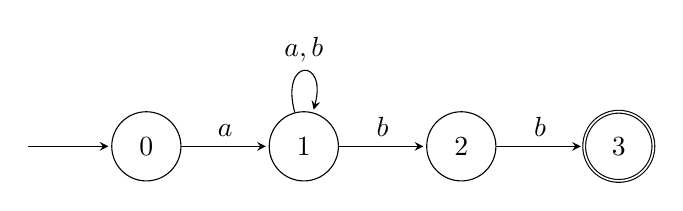
\begin{tikzpicture}[%
    >=stealth,
	shorten >=1pt,
	node distance=2cm,
    auto,
  ]
    \node[state] (0)              {$0$};
    \node[state] (1) [right of=0] {$1$};
    \node[state] (2) [right of=1] {$2$};
    \node[state,double] (3) [right of=2] {$3$};

    \path[->]
    (0) +(-1.5,0) edge (0)
    (0) edge node {$a$} (1)
    (1) edge [loop above] node {$a,b$} ()
    (1) edge node {$b$} (2)
    (2) edge node {$b$} (3)
    ;
  \end{tikzpicture}
\]
\end{simpleexample}

The automaton is \defword{deterministic} (a DFA) iff $\Delta$ is a subset of a function $Q \times \Sigma \rightarrow Q$. I.e., for every state $q \in Q$ and every $a \in \Sigma$, the following state is determined by $\Delta$ or not defined. In that case, we often call the partly-defined function $\delta$ and we write
\[ \A = (Q, \Sigma, q_0, \delta, F). \]

\begin{simpleexample}
\label{reg:dfa-example-1}
The following deterministic automaton is in some way (as defined later) equivalent to the non-deterministic automaton from \cref{reg:nfa-example-1}:
\[
  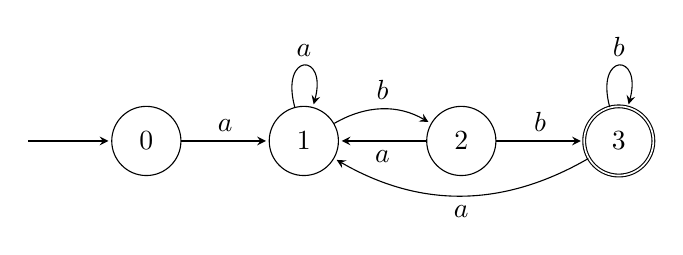
\begin{tikzpicture}[%
    >=stealth,
	shorten >=1pt,
	node distance=2cm,
    auto,
  ]
    \node[state] (0)              {$0$};
    \node[state] (1) [right of=0] {$1$};
    \node[state] (2) [right of=1] {$2$};
    \node[state,double] (3) [right of=2] {$3$};

    \path[->]
    (0) +(-1.5,0) edge (0)
    (0) edge node {$a$} (1)
    (1) edge [loop above] node {$a$} ()
    (1) edge [bend left] node {$b$} (2)
    (2) edge node {$a$} (1)
    (2) edge node {$b$} (3)
    (3) edge [loop above] node {$b$} ()
    (3) edge [bend left] node {$a$} (1)
    ;
  \end{tikzpicture}
\]
\end{simpleexample}

Note that in many cases, as also in \cref{reg:dfa-example-1}, $\delta$ is only a strict subset of a function, i.e. it is not defined on the whole set $Q \times \Sigma$. We call $\A$ \defword{complete}, if $\Delta$/$\delta$ is defined everywhere, i.e. for every state and input symbol, there is a transition defined. If it is not, we can easily extend $\A$ by an additional state, as can be seen in the following example:
\begin{simpleexample}
\label{reg:dfa-example-2}
The automaton from \cref{reg:dfa-example-1} is not complete. This is a complete version of the same automaton:
\[
  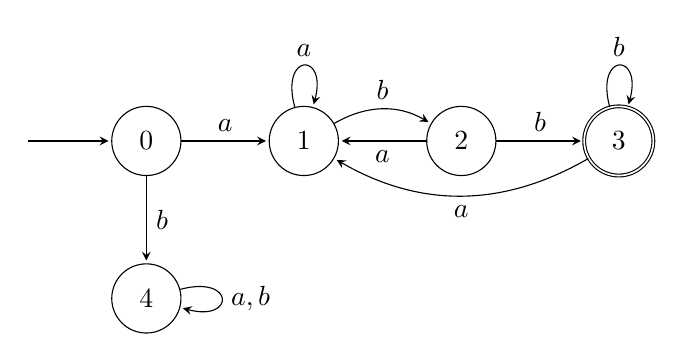
\begin{tikzpicture}[%
    >=stealth,
	shorten >=1pt,
	node distance=2cm,
    auto,
  ]
    \node[state] (0)              {$0$};
    \node[state] (1) [right of=0] {$1$};
    \node[state] (2) [right of=1] {$2$};
    \node[state,double] (3) [right of=2] {$3$};
    \node[state] (4) [below of=0] {$4$};

    \path[->]
    (0) +(-1.5,0) edge (0)
    (0) edge node {$a$} (1)
    (0) edge node {$b$} (4)
    (4) edge [loop right] node {$a,b$} ()
    (1) edge [loop above] node {$a$} ()
    (1) edge [bend left] node {$b$} (2)
    (2) edge node {$a$} (1)
    (2) edge node {$b$} (3)
    (3) edge [loop above] node {$b$} ()
    (3) edge [bend left] node {$a$} (1)
    ;
  \end{tikzpicture}
\]
\end{simpleexample}

Note that we also sometimes have multiple initial states, in which case the automaton is also non-deterministic. Also, in the non-deterministic case, the transition can actual be $\Delta \subseteq Q \times \Sigma^* \times Q$. However, such more generic automaton can be reduced to the definition given here as can be seen in the literature.

Two transitions $(p,a,q), (p',a',q') \in \Delta$ are \defword{consecutive} iff $q=p'$.

A \defword{run} in the automaton $\A$ is a finite sequence of consecutive transitions, written as:
\[ q_0 \xrightarrow{a_0} q_1 \xrightarrow{a_1} q_2 \cdots \]

An automaton $\A = (Q, \Sigma, q_0, \Delta, F)$ \defword{accepts} a finite word $w = (a_0,a_1,\dots,a_n) \in \Sigma^*$ iff there is a run $\rho := q_0 \xrightarrow{a_0} q_1 \xrightarrow{a_1} q_2 \cdots \xrightarrow{a_n} q_{n+1}$ with $q_{n+1} \in F$. We say that the run $\rho$ \defword{matches} the word $w$. We say that the run is an \defword{accepting run}.

The $*$-language $L^*(\A)$ is defined as set of all finite words which are accepted by $\A$.

\begin{simpleexample}
Let $\Sigma = \Set{a,b}$. Let $\A_1 = (Q_1,\Sigma,0,\Delta_1,F_1)$ be the automaton from \cref{reg:nfa-example-1}, $\A_2 = (Q_2,\Sigma,0,\delta_2,F_2)$ be the automaton from \cref{reg:dfa-example-1} and $\A_3 = (Q_3,\Sigma,0,\delta_3,F_3)$ be the automaton from \cref{reg:dfa-example-2}.

For the finite word $w_1 := aabb \in \Sigma^*$, there are three possible runs in $\A_1$:
\begin{enumerate}
\item $0 \xrightarrow{a} 1 \xrightarrow{a} 1 \xrightarrow{b} 1 \xrightarrow{b} 1$
\item $0 \xrightarrow{a} 1 \xrightarrow{a} 1 \xrightarrow{b} 1 \xrightarrow{b} 2$
\item $0 \xrightarrow{a} 1 \xrightarrow{a} 1 \xrightarrow{b} 2 \xrightarrow{b} 3$
\end{enumerate}
The third run is an accepting run because $3 \in F_1$. The other two runs are not accepting. Because there is an accepting run, $w_1 \in L^*(\A_1)$.

In $\A_2$ and $\A_3$, $w_1$ has the deterministic run $0 \xrightarrow{a} 1 \xrightarrow{a} 1 \xrightarrow{b} 2 \xrightarrow{b} 3$. Thus, $w_1 \in L^*(\A_2)$ and $w_1 \in L^*(\A_3)$.

The word $w_2 := aa \in \Sigma^*$ has the only run $0 \xrightarrow{a} 1 \xrightarrow{a} 1$ in $\A_1$, $\A_2$ and $\A_3$. Thus, $w_2 \not\in L^*(\A_1) \cup L^*(\A_2) \cup L^*(\A_3)$.

The word $w_3 := ba \in \Sigma^*$ has no run at all in $\A_1$ and $\A_2$. This demonstrates that $\A_1$ and $\A_2$ are not complete. Thus, $w_2 \not\in L^*(\A_1) \cup L^*(\A_2)$. However, it has the run $0 \xrightarrow{b} 4 \xrightarrow{a} 4$ in $\A_3$. This run doesn't end in an accepting state and there aren't any other runs because $\A_3$ is deterministic, thus $w_3 \not\in L^*(\A_3)$.

We can see that all automata $\A_1$, $\A_2$ and $\A_3$ accept exactly the same words, i.e. the same language. In that sense, they are equivalent.

Informally, they all accept the language of words which start with $a$ and end with $bb$.

A representing regular expression is $a(a+b)^*bb$.
\end{simpleexample}

The class of $*$-languages accepted by a NFA is called $\Lang^*(\text{NFA})$. Likewise, $\Lang^*(\text{DFA})$ is the set of $*$-languages accepted by a DFA. A basic result (see for example \cite{FinAutLogR109} or \cite{InfWordsR110}) is
\[ \Lang^*(\text{DFA}) = \Lang^*(\text{NFA}) = \Lang^*(\text{RE}) . \]
Historically, S.C. Kleene proved in \cite{Kleene56} that $\Lang^*(\text{DFA}) = \Lang^*(\text{RE}) $ and it was shown in \cite{FinAutRabin59} by M. O. Rabin and D. Scott that $\Lang^*(\text{DFA}) = \Lang^*(\text{NFA})$.

This class of $*$-languages is called the class of \defword{regular $*$-languages}. We call it $\Langreg$ from now on.



\subsection{The class of regular $\omega$-languages}
\label{reg-omega-lang}

The class of regular $\omega$-languages can be defined in many different ways. We will use one common definition and show some equivalent descriptions.
\[ \LangOreg := \Set{ \bigcup_{i=1}^n\ U_i \cdot V_i^\omega }{ U_i, V_i \in \Langreg, n \in \N_0 } \]

This is also called the \defword{$\omega$-Kleene closure} of regular languages.

\subsubsection{$\omega$ regular expressions}

For a regular expression $r$ representing a $*$-language $R\subseteq \Sigma^*$, we can introduce a corresponding $\omega$ regular expression $r^\omega$ which represents the $\omega$-language $R^\omega$. This $\omega$ regular expression can be combined with other $\omega$ regular expressions as usual (via union, intersection and complement) and prefixed by standard regular expressions. We call all these combinations $\omega$ regular expressions.

We see that $\LangOreg$ is closed under union (obviously from the definition), intersection and complement.

Thus, the class of languages accepted by $\omega$ regular expressions is exactly $\LangOreg$.


\subsubsection{$\omega$-automata}

A different, very common description is in terms of automata.

An automaton $\A = (Q, \Sigma, q_0, \Delta, F)$ \defword{Büchi-accepts} an infinite word $\alpha = (a_0,a_1,a_2,...) \in \Sigma^\omega$ iff there is an infinite run $q_0 \xrightarrow{a_0} q_1 \xrightarrow{a_1} q_2 \xrightarrow{a_2} q_3 \cdots$ in $\A$ with $\Set{ i \in \N_0 }{ q_i \in F }$ infinite, i.e. which reaches a state in $F$ infinitely often.

The language $L^\omega(\A)$ is defined as the set of all infinite words which are Büchi-accepted by  $\A$. To make clear that we use the Büchi acceptance condition, we sometimes will also write $L^\omega_\text{Büchi}(\A)$.

A basic result of the study of this language class is: The set of all languages accepted by a non-deterministic Büchi automaton is exactly $\LangOreg$ (see \cite{InfCompR101} or others). %S218
Deterministic Büchi automata are less powerful, e.g. they cannot recognise the language $(a+b)^* b^\omega$.

There are some different forms of $\omega$-automata which differ in their acceptance condition. Noteable are the \defword{Muller condition}, the \defword{Rabin condition}, the \defword{Streett condition} and the \defword{Parity condition}. With such an acceptance condition, we call it \defword{Muller automaton}, etc. The \emph{main theorem of $\omega$-automata} states:
\begin{itemize}
\item Non-deterministic Büchi automata,
\item a boolean combination of deterministic Büchi automata,
\item deterministic Muller automata,
\item deterministic Rabin automata,
\item deterministic Streett automata,
\item deterministic Parity automata
\end{itemize}
all recognize the same class of languages. See \cite{InfCompR101}, \cite{LangAutLogicR102}, \cite{InfWordsR110} and others. The main part of this theorem is \defword{McNaughton's Theorem} which states the equivalence of non-deterministic Büchi automata and deterministic Muller automata.
%S407

Muller automata are interesting for us in the rest of this thesis. The acceptance component of a Muller automaton is a set $\F \subseteq 2^Q$, also called the \defword{table} of the automaton (instead of a single set $F \subseteq Q$). A word $w \in \Sigma^\omega$ is accepted iff there is an infinite run $\rho$ with $\Inf(\rho) \in \F$, where $\Inf(\rho)$ is the set of infinitely often reached states of the run $\rho$.

We write:
\[ \A = (Q, \Sigma, q_0, \Delta, \F) . \]

\subsubsection{Language operators}
\label{reg:omega:vialangop}

Büchi acceptance is closely connected to the language operator
\[ \lim(L) := \Set{ \alpha \in \Sigma^\omega }{ \existsinf n \colon \alpha[0,n] \in L } . \]
We define the language class operator
\[ \lim(\Lang) := \Set{\lim(L)}{L \in \Lang} . \]
We see that $\lim(\Langreg)$ is equal to the languages accepted by deterministic Büchi automata (\cite{InfCompR101}). %S407
I.e.
\[ \lim \Langreg = \Set{L^\omega_\text{Büchi}(\A)}{\text{$\A$ is det. Büchi automaton}} . \]
Thus,
\[  \BC \lim \Langreg = \LangOreg , \]
where $\BC \mathcal{X}$ is defined as all \defword{boolean combinations} (union, intersection, complement) from $\mathcal{X}$. Formally: $\BC$ is defined as a function
\[ \BC \colon \Power(\mathcal{W}) \rightarrow \Power(\mathcal{W}) \]
where $\mathcal{W}$ is usually $\Power(\Sigma^\omega)$. Then, $\BC(\mathcal{X})$ is defined as the smallest set with
\begin{itemize}
\item $\mathcal{X} \subseteq \BC \mathcal{X}$,
\item $-X \in \BC \mathcal{X}$ for all $X \in \BC \mathcal{X}$,
\item $X_1 \cup X_2 \in \BC \mathcal{X}$ for all $X_1,X_2 \in \BC \mathcal{X}$,
\item $X_1 \cap X_2 \in \BC \mathcal{X}$ for all $X_1,X_2 \in \BC \mathcal{X}$.
\end{itemize}
$\mathcal{W}$ is always determined from the context. We normally have $\mathcal{W} = \Power(\Sigma^\omega)$, i.e. the set of all $\omega$-languages. Then, $\BC$ is an operator on $\omega$-language classes. We could also have $\mathcal{W} = \Power(\Sigma^*)$, then $\BC$ would be an operator on $*$-language classes. Note that we never have $\mathcal{W} = \Power(\Sigma^* \cup \Sigma^\omega)$ in this thesis. This note is important as the $\BC$ operator would be ambiguous otherwise.

% TODO: ref
Another classification is
\[ \LangOreg = \Set{ \bigcup_{i=0}^n U_i \cdot \lim V_i }{ U_i, V_i \in \Langreg, n \in \N_0 } . \]

\subsubsection{Logic on infinite words}
% TODO: more
%(S218,S411,R107)
Let $L_2(\Sigma)$ be the set of formulas $\operatorname{MSO}(<)$ over $\Sigma$. The interpretation of such formulas over infinite words is straight-forward. In \cite[Theorem 3.1]{CombR107}, we can see that
\[ \LangOreg = \Set{A \subseteq \Sigma^\omega}{A \text{ definable in } L_2(\Sigma)} . \]
% in R107, similar/same thing for Langreg
% In \cite[]{FinAutLogR109}, SOM[+1]

\subsubsection{Some properties}

\begin{lemma}
\label{reg:limRegClosedIntersection}
$\lim \Langreg$ is closed under intersection.
\begin{proof}
In \cite[Chapter 12, Remark 12.4]{CAVR112}, this is shown via a special product automata construction of deterministic Büchi automata.
% one proof, via product automata, would be in http://mtc.epfl.ch/courses/CAV_WS2004/12.pdf
% other sources?
\end{proof}
\end{lemma}

%\section{$* \rightarrow \omega$}

\subsection{Language Operators: Transformation of $*$-languages to $\omega$-languages}

We already introduced $\lim$. We can define a family of language operators, partly also derived from the study of $\LangOreg$. Some of these operators operate on a single language and not on the class. Let $\Lang$ be a $*$-language class. Let $L \in \Lang$.

\begin{enumerate}
\item $\ext(L) := \Set{\alpha \in \Sigma^\omega}{ \exists n \colon \alpha[0,n] \in L} = L \cdot \Sigma^\omega$
\item $\dext(L) := \Set{\alpha \in \Sigma^\omega}{ \forall n \colon \alpha[0,n] \in L}$ (also called the dual-ext)
\item $\BC \ext$
\item $\lim(L) := \Set{ \alpha \in \Sigma^\omega }{ \forall N \colon \exists n > N \colon \alpha[0,n] \in L } = \Set{ \alpha \in \Sigma^\omega }{ \exists^\omega n \colon \alpha[0,n] \in L }$
\item $\dlim(L) := \Set{ \alpha \in \Sigma^\omega }{ \exists N \colon \forall n > N \colon \alpha[0,n] \in L }$ (also called dual-lim)
\item $\BC \lim$
\item $\Kleene(\Lang) := \Set{ \bigcup_{i=1}^n U_i \cdot V_i^\omega}{U_i, V_i \in \Lang, n \in \N_0}$
\item $\limClosure(\Lang) := \Set{\bigcup_{i=1}^n U_i \cdot \lim V_i}{U_i, V_i \in \Lang, n \in \N_0}$
\end{enumerate}

From language operators, we get language class operators in a canonical way, e.g. $\lim(\Lang) := \Set{\lim L}{L \in \Lang}$. $\BC$ denotes always all boolean combinations (union, intersection, complement) of a language class, i.e. for $\mathcal{X} \subseteq \Sigma^\omega \mathbin{\dot\cup} \Sigma^*$, $\BC \mathcal{X}$ is defined as the smallest set such that
\begin{itemize}
\item $\mathcal{X} \subseteq \BC \mathcal{X}$,
\item $-X \in \BC \mathcal{X}$ for all $X \in \BC \mathcal{X}$,
\item $X_1 \cup X_2 \in \BC \mathcal{X}$ for all $X_1,X_2 \in \BC \mathcal{X}$,
\item $X_1 \cap X_2 \in \BC \mathcal{X}$ for all $X_1,X_2 \in \BC \mathcal{X}$.
\end{itemize}

For $\ext$ and $\dext$, we can also introduce equivalent $\omega$ automata acceptance conditions (as in \cite{InfCompR101}). Let $L \subseteq \Sigma^*$ be a regular $*$-language and $\A = (Q, \Sigma, q_0, \Delta, F)$ be an automaton which accepts exactly $L$. Let $\rho$ be an infinte run in $\A$.
\begin{itemize}
\item $\A$ \defword{E-accepts} $\rho$ \ \ iff \ \ $\exists i \colon \rho(i) \in F$,
\item $\A$ \defword{A-accepts} $\rho$ \ \ iff \ \ $\forall i \colon \rho(i) \in F$.
\end{itemize}
We define
\begin{itemize}
\item[] $L^\omega_E(\A) := \Set{\alpha \in \Sigma^\omega}{\text{$\alpha$ is E-accepted in $\A$}}$,
\item[] $L^\omega_A(\A) := \Set{\alpha \in \Sigma^\omega}{\text{$\alpha$ is A-accepted in $\A$}}$,
\end{itemize}
and we have the equalities
\begin{itemize}
\item[] $L^\omega_E(\A) = \ext(L)$,
\item[] $L^\omega_A(\A) = \dext(L)$.
\end{itemize}
Note that $\A$ can be both deterministic or non-deterministic for this property (see \ref{gen:e-determinism}).

\

Given these language operators, we are interested in the relations between them. For the class $\Langreg$ of regular languages, we already know that
\[ \LangOreg = \Kleene(\Langreg) = \BC \lim (\Langreg) = \limClosure(\Langreg) . \]

\subsection{Classification of regular $\omega$-languages} %$\Langreg$

Considering $\Lang := \Langreg$, we get a language diagram like:

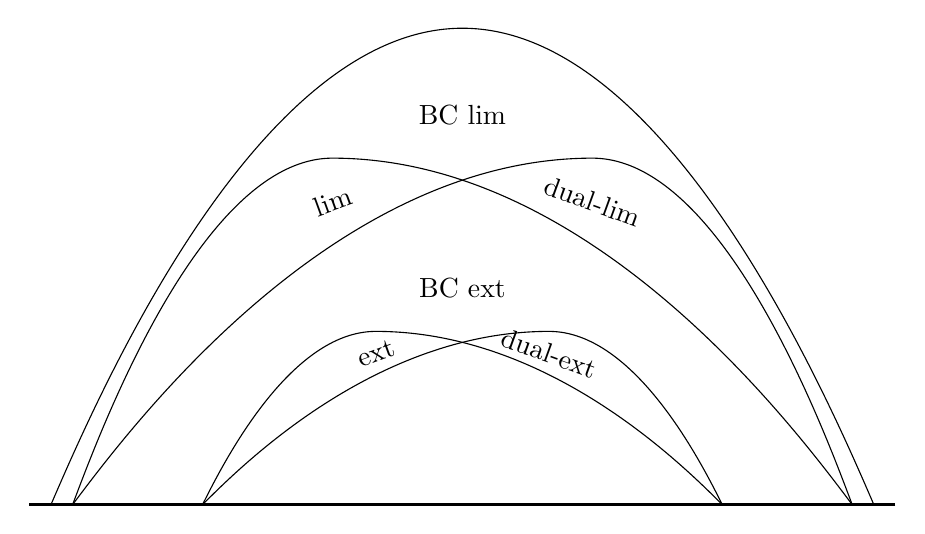
\begin{tikzpicture}
\pgftransformscale{.55}

% http://www.texample.net/tikz/examples/complexity-classes/

%%% HELP LINES - uncomment to design/extend
% \draw[step=1cm,gray,very thin] (-10,0) grid (10,12);
% \node at (0,0) {\textbf{(0,0)}};

%% Horizontal bar
\draw[very thick] (10,0) -- (-10,0);

% BC lim
\draw (-9.5,0) parabola bend (0,11) (9.5,0);
\node at (0,9) {BC lim};

% lim
\draw (-9,0) parabola bend (-3,8) (9,0);
\node[rotate=20] at (-3,7) {lim};

% dual-lim
\draw (-9,0) parabola bend (3,8) (9,0);
\node[rotate=-20] at (3,7) {dual-lim};

% BC ext
%\draw (-6.5,0) parabola bend (0,6) (6.5,0);
\node at (0,5) {BC ext};

% ext
\draw (-6,0) parabola bend (-2,4) (6,0);
\node[rotate=20] at (-2,3.5) {ext};

% dual-ext
\draw (-6,0) parabola bend (2,4) (6,0);
\node[rotate=-20] at (2,3.5) {dual-ext};

\end{tikzpicture}

where all inclusions are strict. In more detail:

% overview of references: S50.1
% S50.2:
\begin{lemma}
\label{P:reg-star}

\begin{enumerate}
\item[1] $\ext \Lang \cap \dext \Lang \neq \emptyset$
\item[2a.] $\ext \Lang \cap \dext \Lang \subsetneqq \ext \Lang$
\item[2b.] $\ext \Lang \cap \dext \Lang \subsetneqq \dext \Lang$
\item[3.] $\ext \Lang \neq \dext \Lang$
\item[4.] $\ext \Lang \cup \dext \Lang \subsetneqq \BC \ext \Lang$
\item[5.] $\BC \ext \Lang = \lim \Lang \cap \dlim \Lang$ (Staiger-Wagner class)
\item[6a.] $\lim \Lang \cap \dlim \Lang \subsetneqq \lim \Lang$
\item[6b.] $\lim \Lang \cap \dlim \Lang \subsetneqq \dlim \Lang$
\item[7.] $\lim \Lang \neq \dlim \Lang$
\item[8.] $\lim \Lang \cup \dlim \Lang \subsetneqq \BC \lim \Lang$
\end{enumerate}
and we have the additional properties
\begin{enumerate}
\item[9.] $\BC \lim \Lang = \Kleene(\Lang)$
\item[10.] $\BC \lim \Lang = \limClosure(\Lang)$
\item[11.] $\BC \lim \Lang = \Set{L_{\text{Büchi}}^\omega(\A)}{\A \text{ automaton so that } L^*(\A) \in \Lang}$
\end{enumerate}

\begin{proof}
\begin{enumerate}
\item[1] $\tilde{L}_1 := a \Sigma^\omega \in \ext \cap \dext \Lang$ with $\tilde{L}_1 = \ext(a)$ and $\tilde{L}_1 = \dext (a \Sigma^*)$. (\cite[prop, p.38]{InfCompR101})
\item[2a.] $\tilde{L}_{2a} := \ext(a^* b) = a^* b \Sigma^\omega \in \ext \Lang$. Assume some A-automaton $\A$ with $n$ states accepts $\tilde{L}_{2a}$. $\A$ would also accept $a^n b^\omega$. I.e. the $(n+1)$th state after the run of $a^n$ would also accept $a$, i.e. $\A$ would accept $a^{n+1}$. By inclusion, $\A$ would accept $a^\omega$. That is a contradiction. Thus, there is no such A-automat. Thus, $\tilde{L}_{2a} \notin \dext \Lang$.
\item[2b.] $\tilde{L}_{2b} := - \tilde{L}_{2a} \in \dext \Lang$, $\tilde{L}_{2b} \notin \ext \Lang$.
\item[3.] Follows directly from P2a and P2b.
\item[4.] $\tilde{L}_4 := \Sigma^* a \Sigma^\omega \cap -(\Sigma^* b \Sigma^\omega)$, $\Sigma = \Set{a,b,c}$. Then we have $\tilde{L}_4 \notin \ext \cup \dext \Lang$, $\tilde{L}_4 \in \BC \ext \Lang$. (\cite[p.38]{InfCompR101})

\item[5.]
%S405 / Staigner-Wagner-recognizable
A language in this class is also said to have the \defword{obligation property}. Staiger and Wagner have introduced a \defword{Staiger-Wagner automaton} (also called a \defword{weak Muller automaton}; see definition \ref{def:staiger-wagner}) which can accept exactly this language class. This class of languages is called the \defword{Staiger-Wagner-recognizable} languages. This is stated in theorem \ref{thm:staiger-wagner}.

%Given an automaton $\A = (Q,\Sigma,q_0,\Delta,\F)$ with $\F \subseteq 2^Q$, a run $\rho$ in $\A$ is \defword{Staiger-Wagner-accepted} iff $\Occ(\rho) \in \F$, where $\Occ(\rho) := \Set{q \in Q}{\text{$q$ occurs in $\rho$}}$.

A generic proof of the equality $\BC \ext \Lang = \lim \Lang \cap \dlim \Lang$ is given in lemma \ref{gen:staiger-wagner}.

\item[6a.] $\tilde{L}_{6a} := \lim(\Sigma^* a) = (\Sigma^* a)^\omega$. Assume there is $L \subseteq \Sigma^*$ with $\lim(L) = -\tilde{L}_{6a}$. Let $(w_0,w_1,w_2,\dotsc) \in (\Sigma^*)^\N$ so that $w_0 \in L, w_0 a w_1 \in L, \dotsc, w_0 \prod_{i=0}^n a w_i \in L \ \forall n \in \N$. Thus, $\alpha := w_0 \prod_{i \in \N} a w_i \in \lim L$. But $\alpha \notin -\tilde{L}_{6a}$. That is a contradiction. Thus, $-\tilde{L}_{6a} \notin \lim \Lang$. Because $\Lang$ is closed under complement, we get $\tilde{L}_{6a} \notin \dlim \Lang$.
\item[6b.] Analog to 6a with $\tilde{L}_{6b} := -\tilde{L}_{6a}$.
\item[7.] Follows directly from 6a and 6b.

\item[8.]
%(S408, S409)
$\tilde{L}_8 := (\Sigma^*a)^\omega \cap -(\Sigma*b)^\omega$. Then $\tilde{L}_8 \notin \lim \cup \dlim \Lang$ but $\tilde{L}_8 \in \BC \lim \Lang$. (\cite[prop, p.38]{InfCompR101})

\item[9.-11.]
%(S402, S407)
%(S403, S411) (R107, Theorem 3.1)
This is explained already in chapter \ref{reg-omega-lang} and in more detail in \cite{InfCompR101} or \cite[Theorem 3.1]{CombR107}.

\end{enumerate}
\end{proof}
\end{lemma}

\subsection{Towards a theory for subclasses of the regular language class} %Questions

This relation diagram was studied in detail for $\Langreg$. We are interested wether we get the same properties for other $*$-language classes under the given language operators.

% \stackrel{?}{\le} or \overset{?}{\le}
%Esp.:
%\begin{itemize}
%\item $\BC \ext \Lang \overset{?}{\subsetneqq} \BC \lim \Lang$
%\end{itemize}

In chapter \ref{general-results}, we will reformulate many proofs of the properties given in chapter \ref{P:reg-star} in a generic way. The results will give us an understanding about when such $\omega$-language class relations hold, when inclusions are strict and when they are not.

These base theorems are then used in chapter \ref{concrete-results} to study some concrete $*$-language classes.

%%!TEX root =  index.tex

% Quelle: Automata, Semigroups, Logic and Games - Pin, Perrin

\section{Automaton}

An \defword{automaton} $\A$ on the alphabet $\Sigma$ is given by a set $Q$ of states and a subset $E \subset Q \times A \times Q$ of transitions. In most cases we also have a subset $I \subset Q$ of initial states and a subset $F \subset Q$ of final states.

We write:
\[ \A = (Q, \Sigma, E, I, F). \]

The automaton is \defword{finite} iff $Q$ and $\Sigma$ are finite.

The automaton is \defword{deterministic} iff $E$ is a set of functions $Q \times A \rightarrow \Q$ and there is only a single initial state.

\subsection{Run}
Two transitions $(p,a,q), (p',a',q') \in E$ are \defword{consecutive} iff $q=p'$.

A \defword{run} in the automaton $\A$ is a sequence of consecutive transitions, written as:
\[ q_0 \rightarrow^{a_0} q_1 \rightarrow^{a_1} q_2 \dots \]

\subsection{Acceptence of finite words}

An automaton $\A = (Q, \Sigma, E, I, F)$ \defword{accepts} a finite word $w = (a_0,a_1,...,a_n) \in \Sigma^*$ iff there is a run $q_0 \rightarrow^{a_0} q_1 \rightarrow^{a_1} q_2 \dots \rightarrow^{a_n} q_{n+1}$ with $q_0 \in I$ und $q_{n+1} \in F$.

The language $L^*(\A)$ is defined as set of all words which are accepted by $\A$.

\section{$*$-languages}
The $*$-languages are all languages of words $w \in \Sigma^*$, i.e. the set of languages of finite words.

\subsection{regular languages}
A languages is \defword{regular} iff an automaton accepts it.

\subsection{piece-wise testable}
\subsection{$k$-locally testable}
\subsection{dot-depth-$n$}
\subsection{starfree}
\subsection{locally modulo testable}
\subsection{$R$-trivial}
\subsection{endlich / co-endlich}
\subsection{endwise testable}

\section{$\omega$-languages}
\subsection{Büchi automaton}
An automaton $\A = (Q, \Sigma, E, I, F)$ \defword{Büchi-accepts} a word $\alpha = (a_0,a_1,a_2,...) \in \Sigma^\omega$ iff there is an infinite run $q_0 \rightarrow^{a_0} q_1 \rightarrow^{a_1} q_2 \rightarrow^{a_2} q_3 ...$ with $q_0 \in I$ and $\{ q_i | q_i \in F \}$ infinite, i.e. which reaches a state in $F$ infinitely often.

The language $L^\omega(\A)$ is defined as the set of all infinite words which are Büchi-accepted by  $\A$.

An automaton $\A$ is a Büchi automaton iff we use the Büchi-acceptence.

\subsection{Muller automaton}
A Muller automaton $\A$ is a finite, deterministic automaton with \defword{Muller acceptence} and a set $\T \in 2^Q$, called the \defword{table} of the automaton (instead of the set $F$). A word $w \in \Sigma^\omega$ is accepted iff there is a run $p$ with $\Inf(p) \in \T$, where $\Inf(p)$ is the set of infinitely often reached states of the run $p$.

We write:
\[ \A = (Q, \Sigma, E, i, \T) . \]

\subsection{Rabin automaton}
A Rabin automaton is a tuple $\A = (Q, \Sigma, E, i, \R)$, where $(Q,\Sigma,E)$ is a deterministic automaton, $i$ is the initial state and $\R = \{(L_j, U_j) | j \in J\}$ is a family of pairs of state-sets. A run $p$ is successfull iff it starts in $i$ and there is an index $j \ in J$ such that $p$ reaches $U_j$ infinitely often and $L_j$ only finitely often. If the automaton is finite, this is equivalent to
\[ \Inf(p) \cap L_j = \emptyset \ \text{and} \ \Inf(p) \cap U_j \neq \emptyset . \]

\subsection{Staiger Wagner class of $\K$}

\section{Operations: $*$-language $K$ to $\omega$-language $L_\omega (K)$}
\subsection{...}
a)
* alle Sprachen $K \dot \Sigma^\omega = \ext(K)$, $K \in \K$

* offene G

* Staiger Wagner Klasse
http://de.wikipedia.org/wiki/Staiger-Wagner-Automat
Erich Grädel, Wolfgang Thomas und Thomas Wilke (Herausgeber), Automata, Logics, and Infinite Games, LNCS 2500, 2002, Seite 20 (auf englisch)
http://www.automata.rwth-aachen.de/material/skripte/areas-english.pdf - s.53

a')
dual $\overline{K}$ = $\omega$-Wörter, deren alle Präfixe in $K$ sind

b) Sprachen $\lim \K$
BC Muller-erkennbare
(BC: boolean closure ?)

b') von einer Stelle an alle Prefixe in $K$

c) Kleene-Closure

alle der Form $\cup_{i=1}^n U_i \dot V_i^\omega$, $U_i, V_i \in \K$

d) $\K$ nicht suffix sensitiv

$K \in \K \Rightarrow K \dot \Sigma^* \in \K$  

\section{General results}
\label{general-results}

%S401: TODO

Let $\Lang$ be a $*$-language class.

\subsection{general}
\label{gen:general}
Let $L,A,B \in \Lang$.
\begin{enumerate}
\item $\ext L = L \cdot \Sigma^\omega$
\item $\ext L = \lim L \cdot \Sigma^*$ %S303
\item $\ext L = \dlim L \cdot \Sigma^*$ %S303, S305.4
\item $- \lim(-L) = \dlim L$
\item $\dlim L \subseteq \lim L$
\item $\lim A \cup \lim B = \lim A \cup B$ \newline %S305.4
Proof:
\begin{align*}
& \alpha \in \lim A \cup \lim B \\
\Leftrightarrow \ & \existsinf n \colon \alpha[0,n] \in A \ \vee \ \existsinf n \colon \alpha[0,n] \in B \\
\Leftrightarrow \ & \existsinf n \colon \alpha[0,n] \in A \cup B \\
\Leftrightarrow \ & \alpha \in \lim A \cup B
\end{align*}
\item $\dlim A \cup \dlim B \subseteq \dlim A \cup B$ \newline %S305.4
Proof:
\begin{align*}
& \alpha \in \dlim A \cup \dlim B \\
\Leftrightarrow \ & \exists N \colon \forall n \ge N \colon \alpha[0,n] \in A \ \vee \ 
\exists N \colon \forall n \ge N \colon \alpha[0,n] \in B \\
\Rightarrow \ & \exists N \colon \forall n \ge N \colon \alpha[0,n] \in A \cup B
\end{align*}
There is no equality in general: $A = (00)^*$, $B = (00)^*0$.
\end{enumerate}

\

%S302.1:
We are interested in relations like $\BC \ext \Lang \overset{?}{\subsetneqq} \BC \lim \Lang$ or $\ext \Lang \overset{?}{\subsetneqq} \lim \Lang$. With $\Lang = \Set{\Set{a}}$, we realize that even $\ext \Lang \subseteq \lim \Lang$ is not true in general ($\ext \Set{\Set{a}} = \Set{a \Sigma^\omega} \neq \emptyset = \lim \Set{\Set{a}}$). In \ref{gen:non-suffix-sens}, we see a sufficient condition for this property, though.

\subsection{non suffix sensitive}
\label{gen:non-suffix-sens}

% S303, S101a:
If E1 ($\forall L \in \Lang \colon L \cdot \Sigma^* \in \Lang$, i.e. $\Lang$ is non suffix sensitive) holds for $\Lang$: For $L \in \Lang$, we have $\ext L = \lim L \Sigma^* = \dlim L \Sigma^*$ and thus
\[ \ext \Lang \subseteq \lim \Lang \cup \dlim \Lang . \]

\subsection{$\BC \ext \subseteq \BC \lim$}
\label{gen:S302a}

%S302:
From $\ext \Lang \subseteq \lim \Lang$, it directly follows $\Set{-\ext L}{L \in \Lang} \subseteq \Set{-\lim L}{L \in \Lang}$. Thus, it also follows
\[ \BC \ext \Lang \subseteq \BC \lim \Lang . \]

\subsection{$\dext \subset \dlim$}

%S302:
From $\ext \Lang \subseteq \lim \Lang$, we need E3 ($\Lang$ closed under negation) to get $\dext \Lang \subseteq \dlim \Lang$. This is in contrast to \ref{gen:S302a}, where it directly follows. We have to be careful about the difference $- \ext \Lang \neq \dext \Lang$ (in general, if E3 does not hold). 

\subsection{union, intersection}
%S303:
\begin{itemize}
\item
E2a (closed under union) $\Rightarrow \bigcup \ext \Lang \subseteq \ext \Lang$.
\item
E2b (closed under intersection) $\Rightarrow \bigcap \ext \Lang \subseteq \ext \Lang$.
\end{itemize}

\subsection{$op \cup \overline{op} \subsetneqq \BC op$}
If there is $L_\Sigma \in \Lang_\Sigma$ with $L_\Sigma \in \ext \Lang_\Sigma, L_\Sigma \not\in \dext \Lang_\Sigma$ and E3 (closed under negation) holds for $\Lang$:
\begin{itemize}
\item[$\Rightarrow$] $-L_\Sigma \in \dext \Lang_\Sigma, -L_\Sigma \not\in \ext \Lang_\Sigma$
\item[$\Rightarrow$] $L_{\Sigma_1} \cup -L_{\Sigma_2} \in \BC \ext \Lang_{\Sigma_1 \dot{\cup} \Sigma_2}$ \newline
$L_{\Sigma_1} \cup -L_{\Sigma_2} \not\in \ext \cup \dext \Lang_{\Sigma_1 \dot{\cup} \Sigma_2}$
\end{itemize}
Thus,
\[ \ext \cup \dext \Lang \subsetneqq \BC \ext \Lang . \]

Similarily, if there is $L_\Sigma \in \lim \Lang_\Sigma, L_\Sigma \not\in \dlim \Lang_\Sigma$ and E3 holds for $\Lang$:
\begin{itemize}
\item[$\Rightarrow$] $-L_\Sigma \in \dlim \Lang_\Sigma, -L_\Sigma \not\in \lim \Lang_\Sigma$
\item[$\Rightarrow$] $L_{\Sigma_1} \cup -L_{\Sigma_2} \in \BC \lim \Lang_{\Sigma_1 \dot{\cup} \Sigma_2}$ \newline
$L_{\Sigma_1} \cup -L_{\Sigma_2} \not\in \lim \cup \dlim \Lang_{\Sigma_1 \dot{\cup} \Sigma_2}$
\end{itemize}
Thus,
\[ \lim \cup \dlim \Lang \subsetneqq \BC \lim \Lang . \]


\subsection{$\BC \ext = \lim \cap \dlim$}
\label{gen:staiger-wagner}
%S405:
A Staiger-Wagner automaton (weak Muller automaton) is of the same form $\A = (Q,\Sigma,q_0,\delta,\F)$ as a Muller automaton with the acceptance condition that a run $\rho$ is accepting if and only if $\Occ(\rho) := \Set{q \in Q \colon \text{q occurs in } p} \in \F$.  (R101,Def.61,p.43)

We see (R101,Th.63+64,p.44) that the class of Staigner-Wagner-recognized languages is exactly the class $\BC \ext \Lang^*(reg)$ and also $\lim \cap \dlim \Lang^*(reg)$.

We are now formulating a more general and direct proof for the $\BC \ext \Lang = \lim \cap \dlim \Lang$ equality without Staiger-Wagner-automata (where some of the ideas are loosely based on (R101,Th.63+64,p.44)).

\

%S305:
First, we show $\lim \cap \dlim \Lang \subseteq \BC \ext \Lang$.

Let $\tilde L \in \lim \cap \dlim \Lang$, i.e. there are deterministic automaton $\A$ and $\overline \A$ so that $L^\omega_{\text{Büchi}}(\A) = L^\omega_{\text{co-Büchi}}(\overline \A) = \tilde L$. Let $Q,\overline Q$ be the states of $\A,\overline \A$. Now look at the product automaton $\A \times \overline \A =: \Ax$ with states $Q \times \overline Q$ and final states $F \times \overline F \subseteq Q \times \overline Q$. $\Ax$ is also deterministic.

%Let $(q,\overline q) \in Q \times \overline F$. If $\overline q$ is not part of a loop in $\A$, we can just take it away from $\overline F$ and get the same $\omega$-language (no matter if Büchi or co-Büchi). Thus assume that all $\overline q \in \overline F$ are part of a loop.

%Let $\alpha \in \tilde L$. Then $\rho(\alpha)$ has infinity many occurences in $F$ and there is some $N$ so that $\overline \rho(\alpha)[N,\infty)$ is only in $\overline F$. Let $\beta \not\in \tilde L$. Then there is some $N$ so that $\rho(\alpha)[N,\infty)$ is only in $Q-F$.

%S305.1
In $\Ax$, we have
\begin{align*}
& \alpha \in \tilde L \\
\Leftrightarrow \ & \forall N \colon \exists n \ge N \colon \overx{\rho}(\alpha)[n] \in F \times \overline Q \\
\Leftrightarrow \ & \exists N \colon \forall n \ge N \colon \overx{\rho}(\alpha)[n] \in Q \times \overline F
\end{align*}

Look at strongly connected component (SCC) $S$ in $\Ax$. We have $S \cap F \times \overline Q \neq \emptyset$, iff $S$ accepts. It follows that all states in $S$ are finite states in $\overline \A$, i.e. $S \cap Q \times \overline F = S$.

Single $\overx{q} \in \overx{Q}$ which are not part of a SCC can be ignored. For the acceptance of infinte words, only SCCs are relevant. For $S$, define $S_+ := \Set{\overx{q} \in \overx{Q}-S}{\overx{q} \text{ can be visited after } S}$.

Then we have
\begin{align*}
\tilde L = \bigcup_{\text{SCC } S} & S \text{ will be visited} \ \wedge \\
& \text{all states of } S \text{ will be visited forever after some step} \ \wedge \\
& S_+ \text{ will not be visited} .
\end{align*}

%S305.2:
$S$ will be visited: Let $S$ exactly be the finite states. This interpreted as an E-automaton $\A^E_S$ is exactly the condition.

Only the allowed states will be visited but nothing followed after $S$: Mark $S$ and all states on all paths to $S$ as finite states. This as an A-automaton $\A^A_S$ is exactly the condition.

A similar negated condition might be simpler: Let $S_+$ be exactly the finite states. Interpret this as an E-automaton $\A^E_{S_+}$.

Then we have
\begin{align*}
\tilde L & = \bigcup_{\text{SCC } S} L^\omega_E (\A^E_S) \cap L^\omega_A (\A^A_S) \\
& = \bigcup_{\text{SCC } S} L^\omega_E (\A^E_S) \cap -L^\omega_E (\A^E_{S_+}) .
\end{align*}

Thus,
\[ \tilde L \in \BC \ext \Lang^*(reg) . \]

%TODO...
Open question at this point: Is $L^*(\A^E_S), L^*(\A^E_{S_+}) \in \Lang$? With E4, this is obviously the case. However, E4 is too strong.

\

%S305.3:
Now let us show $\BC \ext \Lang \subseteq \lim \Lang$.

With E1, we get $\ext \Lang \subseteq \lim \Lang$ and $\ext \Lang \subseteq \dlim \Lang$. I.e. $\ext \Lang \subseteq \lim \cap \dlim \Lang$. Let us show that $\lim \cap \dlim \Lang$ is closed under BC.

Let $\tilde L_a,L_b \in \lim \cap \dlim \Lang$, i.e. $\exists L_{a1}, L_{a2}, L_{b1}, L_{b2} \in \Lang \colon \tilde L_a = \lim L_{a1} = \dlim L_{a2}, \tilde L_b = \lim L_{b1} = \dlim L_{b2}$. Let us show 1. $-\tilde L_a \in \lim \cap \dlim \Lang$, 2. $\tilde L_a \cup \tilde L_b \in \lim \cap \dlim \Lang$.
\begin{enumerate}
\item $-\tilde L_a = -\lim L_{a1} = \dlim -L_{a1}$, $-\tilde L_b = -\dlim L_{a2} = \lim -L_{a2}$. With E3 (closed under negation), we get
\[ -\tilde L_a \in \lim \cap \dlim \Lang . \]

\item
$\tilde L_a \cup \tilde L_b = \lim L_{a1} \cup \lim L_{b1} = \lim L_{a1} \cup L_{b1}$ (\ref{gen:general}). Thus, with E2a, we have
\[ \tilde L_a \cup \tilde L_b \in \lim \Lang . \]

The $\dlim\Lang$ case is harder.
%S305.5: language theoretical proof: TODO
%S305.6:
Let $\A_a$, $\A_b$ be deterministic automaton, so that $L^\omega_{\text{Büchi}}(\A_a) = L^\omega_{\text{co-Büchi}}(\A_a) = \tilde L_a$, $L^\omega_{\text{Büchi}}(\A_b) = L^\omega_{\text{co-Büchi}}(\A_b) = \tilde L_b$. Look at the product automaton $\A_a \times \A_b =: \Ax$. Then we have $L^\omega_{\text{Büchi}}(\Ax) = L^\omega_{\text{co-Büchi}}(\Ax) = \tilde L_a \cup \tilde L_b$.

Thus,
\[ \tilde L_a \cup \tilde L_b \in \dlim \Lang^*(reg) . \]

Open question: Is $L^*(\Ax) \in \Lang$?

\end{enumerate}

%S406.1: TODO...
%S402: TODO...

\subsection{Kleene-star $= \BC \lim$}
\label{gen:kleene-star}
%S407: TODO...
%S306, S306.1:
Let $U,V \in \Lang$. Look at the non-deterministic automaton $\A$ defined as:
\[
  \begin{tikzpicture}[%
    >=stealth,
	shorten >=1pt,
	node distance=2cm,
    auto,
  ]
    \node (U)              {$U$};
    \node (V) [right of=U] {$V \odot$};

    \path[->] (U) +(-1,0) edge (U)
              (U)         edge              node {$\epsilon$} (V)
              (V)         edge  [loop above]       node {} ()
              ;
  \end{tikzpicture}
\]

Then we have $L^\omega_{\text{Büchi}}(\A) = U \cdot V^\omega$.

Let us construct deterministic automata for $\A$ so that we can formulate 'V will be visited and not be left anymore' and 'finite states of the V-related automaton will be visited infinitely often' (or '$UV^*$ will be visited infinitely often').

In a constructed automaton, we must be able to tell wether we are in $U$ or we deterministically have been in $U$ the previous state. In a state power set construction, we can tell wether we are deterministically in $U$ or not. If we are non-determinstic and we may be in both $U$ or $V$ and we get an input symbol which determines that we have been in $U$, we might not be able to tell from the following power set. Example:

Let $U = (a+b)^*$, $V = \Set{b}$. I.e. $UV^\omega = \Set{\alpha \in \Set{a,b}^\omega}{\text{at one point in $\alpha$, there are only $b$s}}$. The non-deterministic automaton is:
\[
  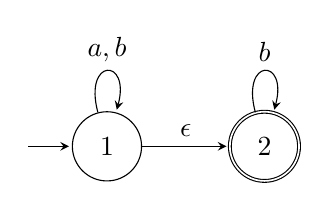
\begin{tikzpicture}[%
    >=stealth,
	shorten >=1pt,
	node distance=2cm,
    auto,
  ]
    \node[state] (1)              {$1$};
    \node[state,double] (2) [right of=1] {$2$};
	
    \path[->]
    (1) +(-1,0) edge (1)
    (1) edge [loop above] node {$a,b$} ()
    (1) edge node {$\epsilon$} (2)
    (2) edge [loop above] node {$b$} ()
    ;
  \end{tikzpicture}
\]

Powerset construction: The initial state is $\Set{1,2}$. Then we have:
\begin{itemize}
\item $\Set{1,2} \overset{a}\rightarrow \Set{1,2}$
\item $\Set{1,2} \overset{b}\rightarrow \Set{1,2}$
\end{itemize}
This gives the $*$-language $\Set{a,b}^*$ and we cannot formulate $UV^\omega$ in any way from there.

In the construction, when we got the $a$ from $\Set{1,2}$, we knew that we have been deterministically in $1$, i.e. in $U$. We loose this information. To keep it, we introduce another state flag which exactly says wether we have determined that we have been in $U$. Thus, we construct an automaton with the states $\Power(Q) \times \B_{\text{det. been in $U$}}$, where $Q$ are the states from $\A$.

For the example, we get the initial state $(\Set{1,2},1)$. Then we have:
\begin{itemize}
\item $(\Set{1,2},1) \overset{a}\rightarrow (\Set{1,2},1)$
\item $(\Set{1,2},1) \overset{b}\rightarrow (\Set{1,2},0)$
\item $(\Set{1,2},0) \overset{a}\rightarrow (\Set{1,2},1)$
\item $(\Set{1,2},0) \overset{b}\rightarrow (\Set{1,2},0)$
\end{itemize}
This is the automaton
\[
  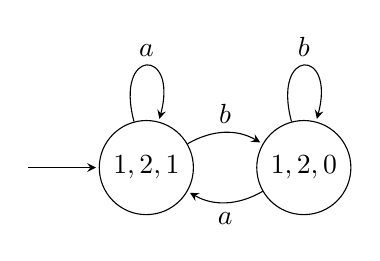
\begin{tikzpicture}[%
    >=stealth,
	shorten >=1pt,
	node distance=2cm,
    auto,
  ]
    \node[state] (1)              {$\Set{1,2},1$};
    \node[state] (2) [right of=1] {$\Set{1,2},0$};

    \path[->]
    (1) +(-1.5,0) edge (1)
    (1) edge [loop above] node {$a$} ()
    (1) edge [bend left] node {$b$} (2)
    (2) edge [bend left] node {$a$} (1)
    (2) edge [loop above] node {$b$} ()
    ;
  \end{tikzpicture}
\]

When we mark all states from $V$ and where we have not been deterministically in $U$ as final, this as a co-Büchi automaton gives exactly the condition 'V will be visited and not be left anymore'. Let $L_E$ be the $*$-language of this automata. Note that $L_E \neq UV^*$ in general and esp. in the example.

When we mark the final states as in the original non-deterministic automata, no matter about $\B_{\text{det. been in $U$}}$, with Büchi-acceptance, we get the condition '$UV^*$ will be visited infinitely often'. This is just $\lim UV^*$.

Together, we get $UV^\omega$, i.e.:
\[ \lim UV^* \cap \dlim L_E = UV^\omega \]

If we have $L_E \in \Lang$, it follows
\[ \Set{ \bigcup_{i=1}^n U_i \cdot V_i^\omega}{U_i, V_i \in \Lang} = \Kleene \Lang \subseteq \BC \lim \Lang . \]

Open question: Is $L_E \in \Lang$?

\

We also need to show $\BC \lim \Lang \subseteq \Kleene \Lang$.

%S306.3:
Show: $\lim \Lang \subseteq \Kleene \Lang$.

Proof: Let $\A$ be a deterministic Büchi automaton for some language $\tilde L = L^\omega_{\text{Büchi}}(\A) \in \Lang$ with final states $F$.

For all finite states $q \in F$: If $q$ is not part of a strongly connected component (SCC), we can ignore it. Let $S$ be the SCC where $q \in S$. Then the set of all $\alpha \in \Sigma^\omega$ which are infinitely often in $q$ can be described as $U_q \cdot V_q^\omega$, where $U_q$ is the set of words so that we arrive in $q$ and $V_q$ is the set of words so that we get from $q$ to $q$. Both sets are regular.

Thus,
\[ \tilde L = L^\omega_{\text{Büchi}}(\A) = \bigcup_{q \in F} U_q V_q^\omega . \]

Obviously, the Kleene-Closure is closed under union.

TODO: Show that Kleene-Closure is closed under negation. (S306.5) (Follows with non-det Büchi complementation but a more generic proof might be useful.)

\subsection{$\Lang(R)$ for a relation $R\subseteq\Sigma^* \times \Sigma^*$}

%S307
If a language class $\Lang(R)$ is defined as finite union of equivalation classes of a relation $R \subseteq \Sigma^* \times \Sigma^*$ and
\begin{itemize}
\item the set of equivalent classes of $R$ is finite,
\item $(v,w) \in R \ \Leftrightarrow \ (va,wa) \in R \ \forall a \in \Sigma$
\end{itemize}
(this is the case for LT, LTT, PT),
then we can construct a canonical deterministic automaton $\A_R$ which has $S_R := \Sigma^* / R$ as states, $\left<\epsilon\right>_R$ is the initial state and the transitions are according to concatenation. Call this an $R$-automaton.

The set of all such $R$-automatoa, varying in the final state set, is isomprophic to $\Lang(R)$. We have
\[ \Lang(R) = \Set{L(\A_R(F))}{F \subseteq S_R} =: \Lang^*(\A_R) . \]

Analogously for $\omega$, we get the set of $R$-E-automata with the $\omega$-language-class
\[ \Lang^\omega_E(\A_R) := \Set{L^\omega(\A^E_R(F))}{F \subseteq S_R} , \]
$R$-Büchi-automata and
\[ \Lang^\omega_{\text{Büchi}} (\A_R) := \Set{L^\omega(\A_R^{\text{Büchi}})}{F \subseteq S_R} , \]
$R$-Muller-automata and
\[ \Lang^\omega_{\text{Muller}} (\A_R) := \Set{L^\omega(\A_R^{\text{Muller}})}{F \subseteq 2^{S_R}} . \]

%S307.1
For a relation $R$ on $\Sigma^*$, there are various ways to construct a relation on $\Sigma^\omega$. For now, we mainly study $R^\omega := \dext R$, i.e.
\[ (\alpha,\beta) \in R^\omega \ :\Leftrightarrow \ \forall n \colon (\alpha[0,n],\beta[0,n]) \in R . \]

Analogously to $\Lang(R)$, define the $\omega$-language-class
\[ \Lang^\omega(R^\omega) := \Set{L^\omega}{\text{$L^\omega$ is finite union of $R^\omega$-equivalence-classes}} . \]

With this preparation, we show for some $R$ the equalities:
\begin{itemize}
\item $\Lang^\omega_E(\A_R) = \ext \Lang(R)$
\item $\Lang^\omega_{\text{Büchi}}(\A_R) = \lim \Lang(R)$
\item $\Lang^\omega_{\text{Muller}}(\A_R) = \BC \lim \Lang(R)$
\item $\Lang^\omega(R^\omega) = \BC \ext \Lang(R)$
\item $\BC \lim \Lang(R) \cap \ext \Lang(reg) = \ext \Lang(R)$
\item $\BC \lim \Lang(R) \cap \lim \Lang(reg) = \lim \Lang(R)$
\item $\lim \Lang(R) \cap \dlim \Lang(R) = \BC \ext \Lang(R)$
\end{itemize}

\subsection{$\Lang^\omega_E(\A_R) = \ext \Lang(R)$}
%S307.2,S307.3
\begin{align*}
& L^\omega = \ext L, L = \bigcup_i \left< w_i\right>_R, L \in \Lang(R) \\
\Leftrightarrow \ & L^\omega = \Set{\alpha \in \Sigma^\omega}{\exists n \colon \alpha[0,n] \in \bigcup_i \left< w_i\right>_R} \\
\Leftrightarrow \ &
\end{align*}


\section{Results on concrete $*$-language classes}
\label{concrete-results}

%\subsection{Overview}
%...
In \cref{chapter:regOmegaLangs}, we already showed many results for the different $\omega$-language classes constructed based on $\Langreg$. Mainly, those are the strict inclusions as shown in the diagram in \cref{regomega-diagram}.

In \cref{general-results}, we found some general conditions on abritrary $*$-language classes $\Lang$ under which the inclusion diagram stays the same. We also gave other conditions on $\Lang$ under which the diagram becomes different or other properties change.

We will now study some concrete well-known $*$-language classes and try to apply the results from \cref{general-results} as well as study some properties individually.

%S15/S151: overview, hierarchy

\subsection{Starfree regular languages}
%S18: def
The set of \defword{star-free $*$-languages} $\Lang(\mathtext{starfree})$ is defined as the smallest set $\Lang = \Lang(\mathtext{starfree})$ with
\begin{itemize}
\item[(a)] $\Set{a} \in \Lang$ for all $a \in \Sigma$,
\item[(b)] $\Lang$ is closed under boolean operations,
\item[(c)] $\Lang$ is closed under concatenation.
\end{itemize}
See \cite[Section 2.2]{ConcHierR104} for further references.

This class is also equivalent to the set of $\mathrm{FO[<]}$-definable languages. %TODO: ref
%W161,S210,S211,S101a,S51
% R107: some characterization
%In \cite[Theorem 3.2]{CombR107}, we see that
%\[  \Lang^\omega(\Set{}) ... \]

First, we start with some specific study on this language class.

%S210:
\begin{theorem}
\[ \Lang^\omega (\mathrm{FO[<]}) = \BC \lim \Lang^*(\mathrm{FO[<]}) \]
\begin{proof}
Let $\varphi \in \mathrm{FO[<]}$. By the \cite[Normal Form Theorem (4.4)]{CombR107} there are bounded formulas $\varphi_1(y),\dotsb,\varphi_r(y),\psi_1(y),\dotsb,\psi_r(y)$ such that for all $\alpha \in \Sigma^\omega$:
\[ \alpha \models \varphi \Leftrightarrow \alpha \models \bigvee_{i=1}^r \left( \forall x \exists y > x \colon \varphi_i (y) \right) \wedge \neg \left( \forall x \exists y > x \colon \psi_i (y) \right) \]
Thus:
\[
\alpha \models \varphi \Leftrightarrow \bigvee_{i=1}^r
\underbrace{ \left( \alpha \models \forall x \exists y > x \colon \varphi_i (y) \right) }_
{\mathclap{\quad\quad \begin{aligned}
& \Leftrightarrow \forall x \exists y > x \colon \alpha[0,n] \models \varphi_i(\omega) \\
& \Leftrightarrow \exists^\omega n \colon \alpha[0,n] \models \varphi_i(\omega) \\
& \Leftrightarrow \alpha \in \lim L^*( \varphi_i(\omega) )
\end{aligned}}}
\wedge \neg \left( \alpha \models \forall x \exists y > x \colon \psi_i (y) \right)
\]
where $\varphi_i(\omega)$ stands for $\varphi_i$ with all bounds removed.
I.e. we have
\[ L^\omega(\varphi) = \bigcup_{i=1}^r \lim( L^* (\varphi_i (\omega)) \cap \neg \lim( L^* (\psi_i (\omega))) , \]
and thus
\[ L^\omega(\varphi) \in \BC \lim \Lang^* (\mathrm{FO[<]}) . \]
We have prooved the $\subseteq$-direction. For $\supseteq$:
\begin{align*}
& \alpha \in \lim( L^*(\varphi) ) \\
\Leftrightarrow \ & \exists^\omega n \colon \alpha[0,n] \models \varphi \\
\Leftrightarrow \ & \alpha \models \forall x \exists y > x \colon \varphi(y) \\
\Leftrightarrow \ & \alpha \in L^\omega ( \forall \exists y > x \colon \varphi(y) )
\end{align*}
where $\varphi(y)$ stands for $\varphi$ with all variables bounded by $y$.
I.e.
\[ \lim \Lang^* (\mathrm{FO[<]}) \subseteq \Lang^\omega (\mathrm{FO[<]}) , \]
and thus also
\[ \BC \lim \Lang^* (\mathrm{FO[<]}) \subseteq \Lang^\omega (\mathrm{FO[<]}) . \]
Thus we have prooved the equality.
\end{proof}
\end{theorem}

%S211:
\begin{theorem}
\[ \BC \ext \Lang^*( \mathrm{FO[<]} ) \subsetneqq \BC \lim \Lang^* ( \mathrm{FO[<]} ) \]
\begin{proof}
$\subseteq$: $L \subset \Sigma^\omega \text{ starfree } \ \Rightarrow\ L \Sigma^\omega \in \lim( \Lang^*( \mathrm{FO[<]} ) )$

$\neq$:
\begin{align*}
& L := (\Sigma^* a)^\omega \\
\Rightarrow \ & L = \lim( (\Sigma^* a)^* ) \\
\Rightarrow \ & L = L^\omega(\exists^\omega x : Q_a x)
\end{align*}
And we have $L \notin \BC \ext \Lang^* (\mathrm{FO[<]})$.
\end{proof}
\end{theorem}

%S101a:
$\Set{a} \in \Lang$. $a \Sigma^* \in \Lang$, thus $a\Sigma^\omega = \ext(\Set{a}) = \dext{a\Sigma^*}$. I.e. $\ext \cap \dext \Lang \ne \emptyset$.

$\Lang^*( \mathrm{FO[<]} )$ is obviously \emph{closed under negation, suffix-independence, union and alphabet permutation}.

We can also see that $\Lang^*( \mathrm{FO[<]} )$ is \emph{closed under change of final states}. %TODO: argue

$L_a := \Sigma^* a \in \Lang$ is a $\ext$-$\dext$-separating and $\lim$-$\dlim$-separating language.

Thus, with \cref{gen:main-theorem-inclusions}, we get
\[ \ext \cap \dext \Lang \subsetneqq
\ext \cup \dext \Lang \subsetneqq
\BC \ext \Lang =
\lim \cap \dlim \Lang \subsetneqq
\lim \cup \dlim \Lang \subsetneqq
\BC \lim \Lang . \]


\subsection{Piecewise testable languages}
%S19: def
\label{lang:PT}
Let $u,v \in \Sigma^*$. For $n \in \N$, define the congruence relation $\simeq_{\PT_n}$:
\[ u \simeq_{\PT_n} v \ \ \ :\Leftrightarrow \ \ \ \operatorname{Subwords}_{\le n}(u) = \operatorname{Subwords}_{\le n}(v) , \]
where
\[ \operatorname{Subwords}_{\le n}(u) := \Set{w \in \Sigma^{\le n}}{\text{$w$ is a subword of $u$}} \]
and $w$ is a \defword{subword} of $u$ for $w,u \in \Sigma^*$ iff there is a subsequence $(s_n)_{n\in\N}$ of $(n)_{n\in\N}$ such that $w = u|_s$.

Define
\[ \Lang(\PT_n) := \Lang(\simeq_{\PT_n}). \]
Then the class of \defword{piecewise testable languages} is defined as
\[ \Lang(\PT) := \bigcup_{n\in\N} \Lang(\PT) . \]

We also have the characterization
\[ \Lang(\PT) = \BC \bigcup_{n\in\N_0,a_i \in \Sigma} \Set{\Sigma^* a_1 \Sigma^* a_2 \Sigma^* \cdots\Sigma^* a_n \Sigma^*} . \]
% The syntactic monoid is also J-trivial.

See \cite[Section 2.3]{ConcHierR104} for further references.

%S52: overview
%S212: BC lim class

$L$ piece-wise testable $\Leftrightarrow$ $L$ is a boolean algebra of $\Sigma^* a_1 \Sigma^* a_2 \dotsb a_n \Sigma^*$.

%S101:
\begin{theorem}
\label{thm.PT}
\[ \BC \ext \Lang^* (\PT) = \BC \lim \Lang^* (\PT) \]
\begin{proof}
$\subseteq$: It is sufficient to show $\ext(\Lang^* (\PT)) \subseteq \BC \lim \Lang^* (\PT)$.

By complete induction:
\begin{align*}
& \ext(\Sigma^* a_1 \Sigma^* a_2 \dotsb a_n \Sigma^*) = \Sigma^* a_1 \Sigma^* a_2 \dotsb a_n \Sigma^\omega = \lim(\Sigma^* a_1 \Sigma^* a_2 \dotsb a_n \Sigma^*) \\
& \ext( \neg ( \Sigma^* a_1 \Sigma^* a_2 \dotsb a_n \Sigma^* )) = \Sigma^\omega = \lim( \Sigma^* ) \\
& \ext( \emptyset ) = \emptyset = \lim(\emptyset)
\end{align*}

It is sufficient to show negation only for such ground terms because we can always push the negation down.
\begin{align*}
& \ext(A \cup B) = \ext(A) \cup \ext(B) \\
& \ext(A \cap B) = \ext(A) \cap \ext(B)
\end{align*}

This makes the induction complete.

$\supseteq$: It is sufficient to show $\lim(\Lang^* (\PT)) \subseteq \BC \ext \Lang^* (\PT)$.
\begin{align*}
& \lim(\emptyset) = \ext(\emptyset), \ \lim(\Sigma^* a_1 \Sigma^* a_2 \dotsb a_n \Sigma^*) = \ext(\Sigma^* a_1 \Sigma^* a_2 \dotsb a_n \Sigma^*) \ \ \text{(see above)} \\
& \begin{aligned}
\lim( \neg ( \Sigma^* a_1 \Sigma^* a_2 \dotsb a_n \Sigma^* ) ) & = \Set{ \alpha \in \Sigma^\omega }{ \exists^\omega n \colon \alpha [0,n] \notin \Sigma^* a_1 \Sigma^* a_2 \dotsb a_n \Sigma^* } \\
& = \Set{ \alpha \in \Sigma^\omega }{ \forall n \colon \alpha [0,n] \notin \Sigma^* a_1 \Sigma^* a_2 \dotsb a_n \Sigma^* } \\
& = \neg \ext( \Sigma^* a_1 \Sigma^* a_2 \dotsb a_n \Sigma^* )
\end{aligned} \\
& \begin{aligned}
\lim(A \cup B) & = \Set{ \alpha \in \Sigma^\omega }{ \exists^\omega n \colon \alpha[0,n] \in A \cup B } = \lim(A) \cup \lim(B) \\
\lim(A \cap B) & = \Set{ \alpha \in \Sigma^\omega }{ \exists^\omega n \colon \alpha[0,n] \in A \cap B } \\
\intertext{and because $A,B$ are piece-wise testable}
& = \Set{ \alpha \in \Sigma^\omega }{ \exists n : \forall m > n \colon \alpha[0,m] \in A \cap B } = \lim(A) \cap \lim(B)
\end{aligned}
\end{align*}
\end{proof}
\end{theorem}



\label{lang:posPT}
\defword{Positive piece-wise testable languages} are defined as
\[ \Lang(\mathtext{pos-PT}) := \operatorname{pos-BC} \bigcup_{n\in\N_0,a_i \in \Sigma} \Set{\Sigma^* a_1 \Sigma^* a_2 \Sigma^* \cdots\Sigma^* a_n \Sigma^*} . \]

For positive piece-wise testable (pos-PT) languages, we get the same result.
%\subsection{positive piece-wise testable}
%S53: overview
%S214: BC lim class

%S101:
\begin{theorem}
\label{thm.ext.lim.posPT}
\[ \BC \ext \Lang^* (\mathtext{pos-PT}) = \BC \lim \Lang^* (\mathtext{pos-PT}) \]
\begin{proof}
$\subseteq$: Exactly like the proof for PT except that we leave out the negated part.

$\supseteq$: Also like the proof for PT.
\end{proof}
\end{theorem}

We also have a relation between pos-PT and PT.

\begin{theorem}
\[ \BC \ext \Lang^*(\mathtext{pos-PT}) = \BC \ext \Lang^* (\mathtext{PT}) \]

\begin{proof}
In the proof of $\lim \Lang^*(\mathtext{PT}) \subseteq \BC \ext \Lang^* (\mathtext{PT})$ we actually proved $\BC \lim \Lang^*(\mathtext{PT}) \subseteq \BC \ext \Lang^* (\mathtext{pos-PT})$. Similiarly we also proved $\BC \ext \Lang^* (\mathtext{PT}) \subseteq \BC \lim \Lang^* (\mathtext{pos-PT})$.

With \cref{thm.PT} and \cref{thm.ext.lim.posPT} we get the claimed equality.
\end{proof}
\end{theorem}


\subsection{Locally testable languages}
\label{lang:LT}
%S16: def
Let $u,v \in \Sigma^*$. For $n \in \N$, define the congruence relation $\simeq_{\text{LT}_n}$:
\begin{alignat*}{3}
u \simeq_{\text{LT}_n} v \ \ \ && :\Leftrightarrow \ \ \ & \operatorname{left-Fact}_{<n}(u) = \operatorname{left-Fact}_{<n}(v) , \\
&&& \operatorname{right-Fact}_{<n}(u) = \operatorname{right-Fact}_{<n}(v) , \\
&&& \operatorname{Fact}_{n}(u) = \operatorname{Fact}_{n}(v) \\
&& \Leftrightarrow \ \ \ & u \simeq_{\text{endwise}_n} v , \\
&&& \operatorname{Fact}_n(u) = \operatorname{Fact}_n(v)
\end{alignat*}
where
\begin{align*}
\operatorname{left-Fact}_{<n}(v) & := \Set{w \in \Sigma^{<n}}{\text{$w$ is left-factor of $v$}} \\
\operatorname{right-Fact}_{<n}(v) & := \Set{w \in \Sigma^{<n}}{\text{$w$ is right-factor of $v$}} \\
\operatorname{Fact}_{n}(v) & := \Set{w \in \Sigma^{n}}{\text{$w$ is factor of $v$}}.
\end{align*}
For $v,w \in \Sigma^*$,
\begin{align*}
\text{$w$ is a \defword{left-factor} of $v$} & \ :\Leftrightarrow \ \exists u \in \Sigma^* \colon wu = v \\
\text{$w$ is a \defword{right-factor} of $v$} & \ :\Leftrightarrow \ \exists u \in \Sigma^* \colon uw = v \\
\text{$w$ is a \defword{factor} of $v$} & \ :\Leftrightarrow \ \exists u_1,u_2 \in \Sigma^* \colon u_1 w u_2 = v.
\end{align*}

Define
\[ \Lang(\LT_n) := \Lang(\simeq_{\text{LT}_n}) . \]
Then the class of \defword{locally testable languages} is defined as
\[ \Lang(\LT) := \bigcup_{n\in\N} \Lang(\LT_n) . \]

We also have the characterization
\[ \Lang(\LT) = \BC \bigcup_{u,v,w \in \Sigma^+} \Set{u\Sigma^*, \Sigma^* v, \Sigma^* w \Sigma^*, \Set{\epsilon}} . \]

See \cite[Section 2.5]{ConcHierR104} for further references.

\begin{theorem}
\[ \BC \ext \Lang^* (\LT) \subsetneqq \BC \lim \Lang^*(\LT)  \]

\begin{proof}
Let $w \in \Sigma^+$.
\begin{align*}
& \ext (w \Sigma^*) = \lim(w \Sigma^*) \\
& \ext( \Sigma^* w) = \Sigma^* w \Sigma^\omega = \lim( \Sigma^* w \Sigma^* ) \\
& \ext( \Sigma^* w \Sigma^*) = \Sigma^* w \Sigma^\omega = \lim( \Sigma^* w \Sigma^* )
\end{align*}
Thus we have
\[ \BC \ext \Lang^* (\LT) \subseteq \BC \lim \Lang^*(\LT) . \]
But we also have
\[ \lim(\Sigma^*) = (\Sigma^* w)^\omega \notin \BC \ext \Lang^* (\LT) . \]
\end{proof}
\end{theorem}

% TODO: I think R105... handles them?
\defword{Positive locally testable languages} are defined as
\[ \Lang(\mathtext{pos-LT}) = \operatorname{pos-BC} \bigcup_{u,v,w \in \Sigma^+} \Set{u\Sigma^*, \Sigma^* v, \Sigma^* w \Sigma^*, \Set{\epsilon}} . \]

\subsection{Locally threshold testable languages}
\label{lang:LTT}
%S17: def
% FinAutLogR109
Let $u,v \in \Sigma^*$. Let $k,r \in \N$, define the congruence relation $\simeq_{\text{LTT}^k_r}$:
\begin{alignat*}{3}
u \simeq_{\text{LTT}^k_r} v \ \ \ && :\Leftrightarrow \ \ \ & \operatorname{left-Fact}_{<n}(u) = \operatorname{left-Fact}_{<n}(v) , \\
&&& \operatorname{right-Fact}_{<n}(u) = \operatorname{right-Fact}_{<n}(v) , \\
&&& \begin{aligned}
\forall x \in \Sigma^{\le k} \colon & \operatorname{count-Fact}_x(u) = \operatorname{count-Fact}_x(v) < r \ \ \ \ \text{or} \\
& \min \Set{\operatorname{count-Fact}_x(u), \operatorname{count-Fact}_x(v)} \ge r
\end{aligned}
\end{alignat*}
where for $x \in \Sigma^*$, $\operatorname{count-Fact}_x(u)$ states how often $x$ occurs as a factor in $u$, formally
\[ \operatorname{count-Fact}_x(u) := \#\Set{n \in \N}{u[n,n+\vert x \vert - 1] = x} . \]
Define
\[ \Lang(\text{LTT}^k_r) := \Lang(\simeq_{\text{LTT}^k_r}). \]
Then the class of \defword{locally threshold testable languages} is defined as
\[ \Lang(\mathtext{LTT}) := \bigcup_{k,r\in\N} \Lang(\text{LTT}^k_r) . \]

Locally threshold testable languages are a generalization of locally testable language. We can see that
\[  \Lang(\LT) = \bigcup_{k\in\N} \Lang(\text{LTT}^k_1) . \]

For further references, see \cite[IV.3]{FinAutLogR109}.

In \cite[IV.3.3]{FinAutLogR109}, we can see that
\[  \Lang(\text{LTT}) = \Lang(\mathrm{FO[+1]}). \]
%\subsection{FO[+1]}
%def: S17
%S213: BC ext class
%215: BC lim class

%S103:
\begin{theorem}
\[ \Lang^\omega (\mathrm{FO[+1]}) = \BC \ext \Lang^*(\mathrm{FO[+1]}) \]
\begin{proof}
From \cite[Theorem 4.8]{LangAutLogicR102}, we know that each formular in FO[+1] is equivalent (for both finite and infinite words) to a boolean combination of statements ``sphere $\sigma \in \Sigma^+$ occurs $\geq n$ times''. That statement can be expressed by a sentence of the form
\[ \psi := \exists \overline{x_1} \dotsb \exists \overline{x_n} \varphi(\overline{x_1}, \dotsb, \overline{x_n}) \]
where each $\overline{x_i}$ is a $\abs{\sigma}$-tuple of variables and the formula $\varphi$ states:
\[
\bigwedge_{\mathclap{i,j \in \underline{n},\atop { i \neq j,\atop k,l \in \underline{\abs{\sigma}}}}} x_{i,k} \neq x_{j,l}
\ \wedge\ \bigwedge_{\mathclap{i \in \underline{n},\atop k \in \underline{\abs{\sigma}-1}}} x_{i,k+1} = x_{i,k} + 1
\ \wedge\ \bigwedge_{\mathclap{i \in \underline{n},\atop k \in \underline{\abs{\sigma}}}} Q_{\sigma_k} x_{i,k}
\]
For $\psi$, we have:
\[ \alpha \models \psi \Leftrightarrow \exists n \colon \alpha[0,n] \models \psi \ \ \text{for all } \alpha \in \Sigma^\omega , \]
i.e.
\[ L^\omega(\psi) = \ext L^*(\psi) . \]
Any formular in FO[+1] can be expressed as a boolean combination of $\psi$-like formular. With
\begin{align*}
& L^\omega(\neg \psi) = \neg L^\omega(\psi) \\
& L^\omega(\psi_1 \wedge \psi_2) = L^\omega(\psi_1) \cap L^\omega(\psi_2) \\
& L^\omega(\psi_1 \vee \psi_2) = L^\omega(\psi_1) \cup L^\omega(\psi_2)
\end{align*}
we get:
\[ \Lang^\omega(\mathrm{FO[+1]}) = \BC \ext \Lang^*(\mathrm{FO[+1]}). \]
\end{proof}
\end{theorem}

\subsection{FO[]}

\subsection{Endwise testable languages}
\label{lang:endwise}
%S20: def
Let $u,v \in \Sigma^*$. For $n \in \N$, define the congruence relation $\simeq_{\text{endwise}_n}$:
\begin{alignat*}{3}
u \simeq_{\text{endwise}_n} v \ \ \ && :\Leftrightarrow \ \ \ & \operatorname{left-Fact}_{<n}(u) = \operatorname{left-Fact}_{<n}(v) , \\
&&& \operatorname{right-Fact}_{<n}(u) = \operatorname{right-Fact}_{<n}(v)
\end{alignat*}
Then the class of \defword{endwise testable languages} is defined as
\[ \Lang(\mathtext{endwise}) := \bigcup_{n\in\N} \Lang(\simeq_{\text{endwise}_n}) . \]

We also have the characterization
\[ \Lang(\mathtext{endwise}) = \Set{X \Sigma^* Y \cup Z}{X,Y \subseteq \Sigma^+, Z \subseteq \Sigma^*, \text{$X,Y,Z$ finite}} . \]

See \cite[Section 2.4]{ConcHierR104} for further references.

%S104:
\begin{itemize}
\item $\BC \ext \Lang^*(\mathtext{endwise}) \neq \BC \lim \Lang^*(\mathtext{endwise})$ because $\Sigma^*a \in \Lang^*(\mathtext{endwise})$.
\item $\ext(a\Sigma^* a) = a \Sigma^* a \Sigma^\omega \notin \BC \lim \Lang^*(\mathtext{endwise})$
\end{itemize}

\subsection{Local languages}
\label{lang:local}

\subsection{Finite / Co-finite languages}
\label{lang:finite}
%S105:
\begin{itemize}
\item $\lim \Lang^*(\mathtext{finite}) = \Set{\emptyset}$
\item $\ext \Lang^*(\mathtext{finite}) = \Lang^*(finite) \cdot \Sigma^\omega$
\item $\lim \Lang^*(\mathtext{co-finite}) = \Set{\Sigma^\omega}$
\item $\ext \Lang^*(\mathtext{co-finite}) = \Set{\Sigma^\omega}$
\end{itemize}

\subsection{Regular languages of dot-depth-$n$}
\label{lang:dotdepth}
%S21: def

\subsection{$L$-trivial languages}
\label{lang:Ltrivial}
\subsection{$R$-trivial languages}
\label{lang:Rtrivial}
%S23: def
\subsection{Locally modulo testable languages}
\label{lang:LmodT}
%S24: def

%\subsection{$k$-locally testable}

\subsection{Context free languages}
\label{lang:contextfree}



%!TEX root =  index.tex
\section{Conclusion}
\label{chapter:conclusion}

Via language class operators like $\ext$ or $\lim$, we induced $\omega$-language classes from $*$-language classes. We presented the known results on the relations of the induced $\omega$-lanugage classes from $\Langreg$. Those relations were shown in the diagram in \cref{regomega-diagram}.

Then, we worked on several generic cases on arbitrary $*$-language classes $\Lang$ such that we get the expected inclusions as in the diagram or at least some of them. However, we have also seen several examples where we have different relations. We introduced some closure properties on $\Lang$ which lead to the expected results. The closure under negation, union or intersection is given for most $*$-language classes. Important for some relations, e.g. the $\BC \ext \Lang = \lim \cap \dlim \Lang$ is the closure under change of final states. This property had to be adjusted several times to be powerful enough so that the proofs worked and that it still applied to important language classes such as starfree languages or all the congruence based language classes.

In \cref{gen:section:kleene}, we studied the relation between $\BC \lim \Lang$ and $\Kleene \Lang$. We saw that the equality as for $\Langreg$ didn't easily followed in the generic case with any of the given introduced closure properties on $\Lang$. Thus, finding better properties on $\Lang$ for when the equality or inclusion in some direction holds is open for future research.

In \cref{gen:R}, we have seen that congruence based language classes gives us many nice properties which makes arguing about the induced $\omega$-languages classes easy. However, as many important language classes are not based on congruences, namely the starfree languages or the whole class of regular languages, we cannot directly apply the results in many cases. Even in the case for locally testable languages or piecewise testable languages, we can only directly apply the results for the given $\LT_n$ or $\PT_n$ relation but not for the whole class $\LT$ or $\PT$. A possible generalization for the section would be if we have a class of $\Lang$-automata instead of a single $\Lang$-automata. In the case of $\PT$, this would be $\bigcup_n \text{$\PT_n$-automata}$. In \cref{lang:PT}, we actually see this applied.

In \cref{concrete-results}, we studied some of the most well-known subclasses of the class of regular $*$-languages. There are many more regular language subclasses like local languages, $L$-trivial or $R$-trivial languages or locally modulo testable languages. On all these classes, we can probably apply some of the results from \cref{general-results}.

Also interesting are supersets of the class of regular $*$-languages. One important class are the context-free languages. Also deterministic context-free languages or context-sensitive languages might be interesting to study in this context. A starting point to study these classes are to extend the results from \cref{general-results} to pushdown automata or other more generic cases.

Also interesting are further variations of the presented language classes, such as their only-positive variants (like $\posPT$).

Overall, we developed some powerful theorems but many questions or ideas remain open for future work.


\section{References}
% http://www.automata.rwth-aachen.de/material/skripte/latex/latex.pdf
% 9.2ff
\bibliographystyle{alpha}
\bibliography{bibliography}

\printindex

\end{document}
